% This text is proprietary.
% It's a part of presentation made by myself.
% It may not used commercial.
% The noncommercial use such as private and study is free
% Sep. 2005 
% Author: Sascha Frank 
% University Freiburg 
% www.informatik.uni-freiburg.de/~frank/


\documentclass{beamer}

\usepackage{graphicx}

\begin{document}
\title{Simple Beamer Class}   
\author{Sascha Frank} 
\date{\today} 

\frame{\titlepage} 

\frame{\frametitle{Table of contents}\tableofcontents} 

\section{Usando Branchs} 

\frame{\frametitle{Exemplo} 
\begin{figure}[h!]
\centering
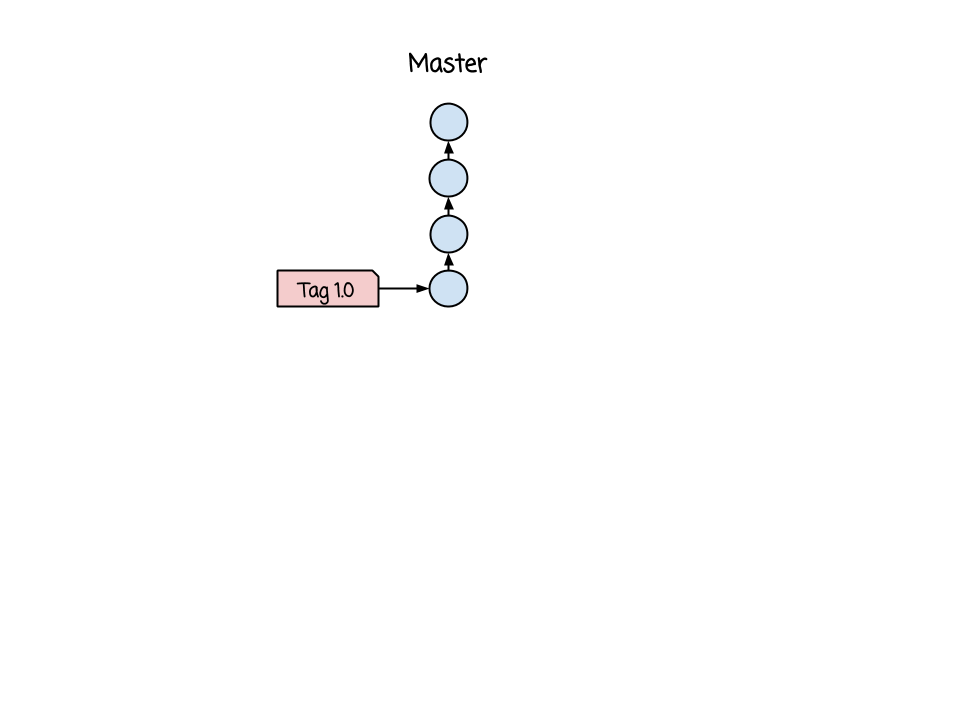
\includegraphics[width=1\textwidth]{img/exemplo-01}
\end{figure}
}

\frame{\frametitle{Exemplo} 
\begin{figure}[h!]
\centering
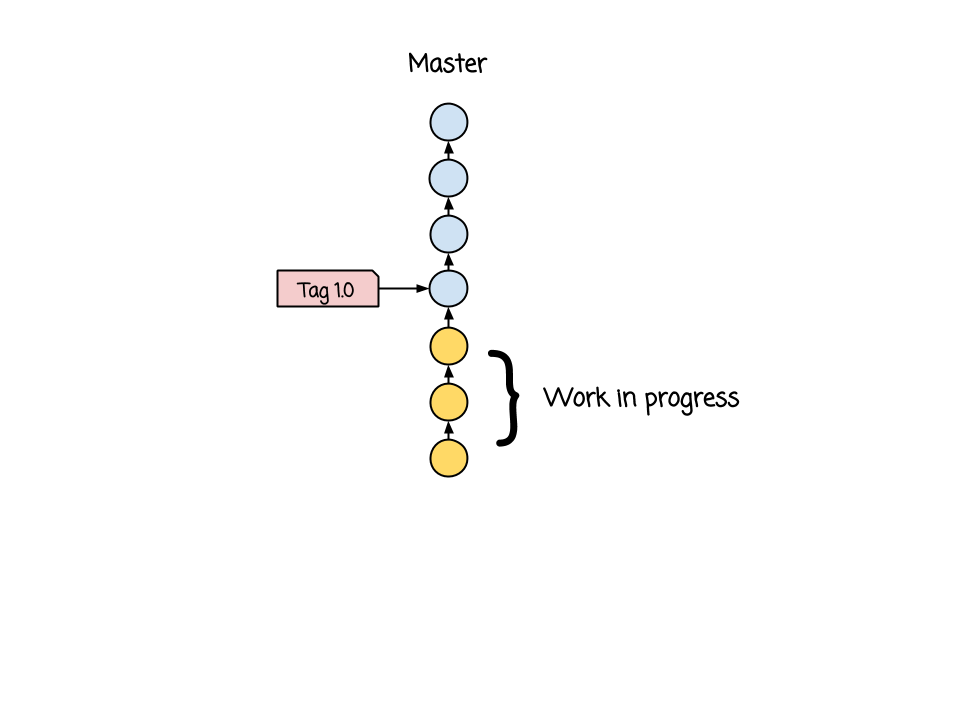
\includegraphics[width=1\textwidth]{img/exemplo-02}
\end{figure}
}

\frame{\frametitle{Exemplo} 
\begin{figure}[h!]
\centering
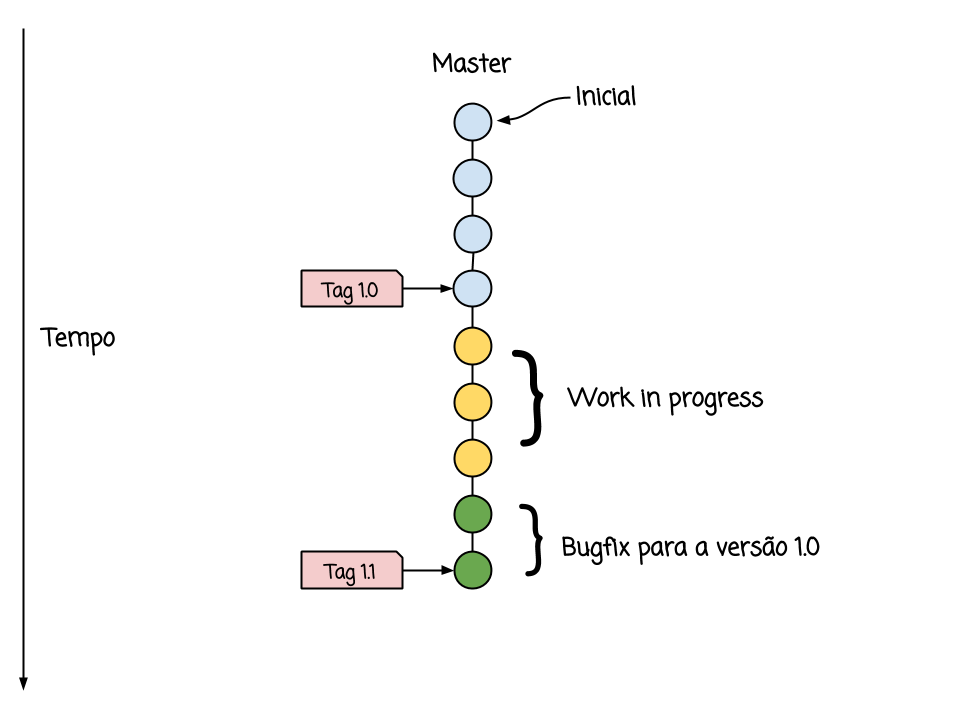
\includegraphics[width=1\textwidth]{img/exemplo-03}
\end{figure}
}

\frame{\frametitle{Exemplo} 
\begin{figure}[h!]
\centering
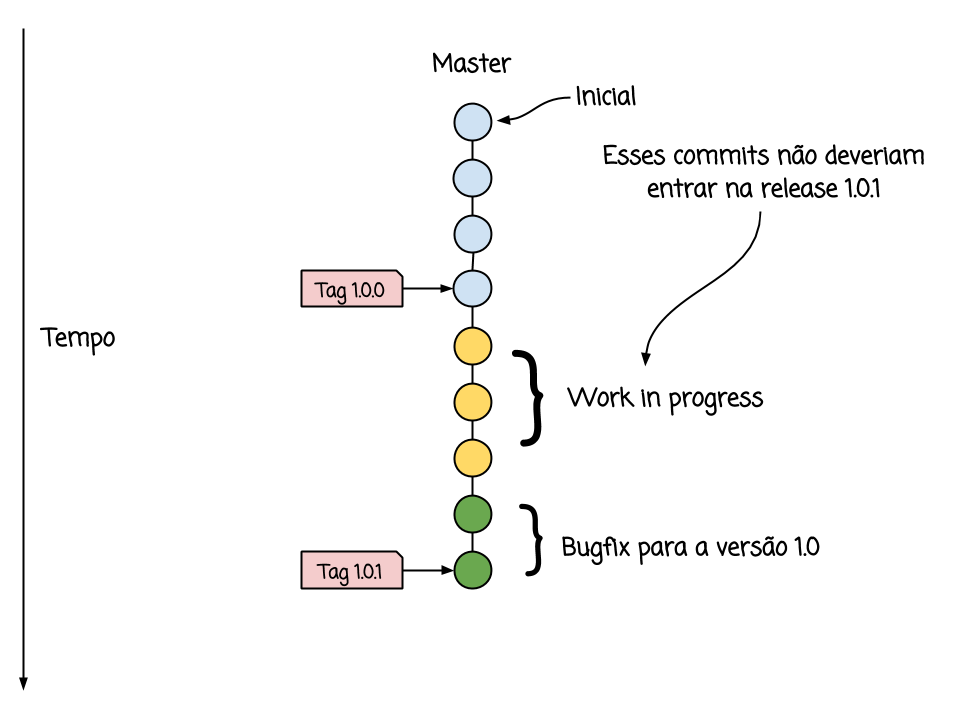
\includegraphics[width=1\textwidth]{img/exemplo-04}
\end{figure}
}

\frame{\frametitle{Exemplo} 
\begin{figure}[h!]
\centering
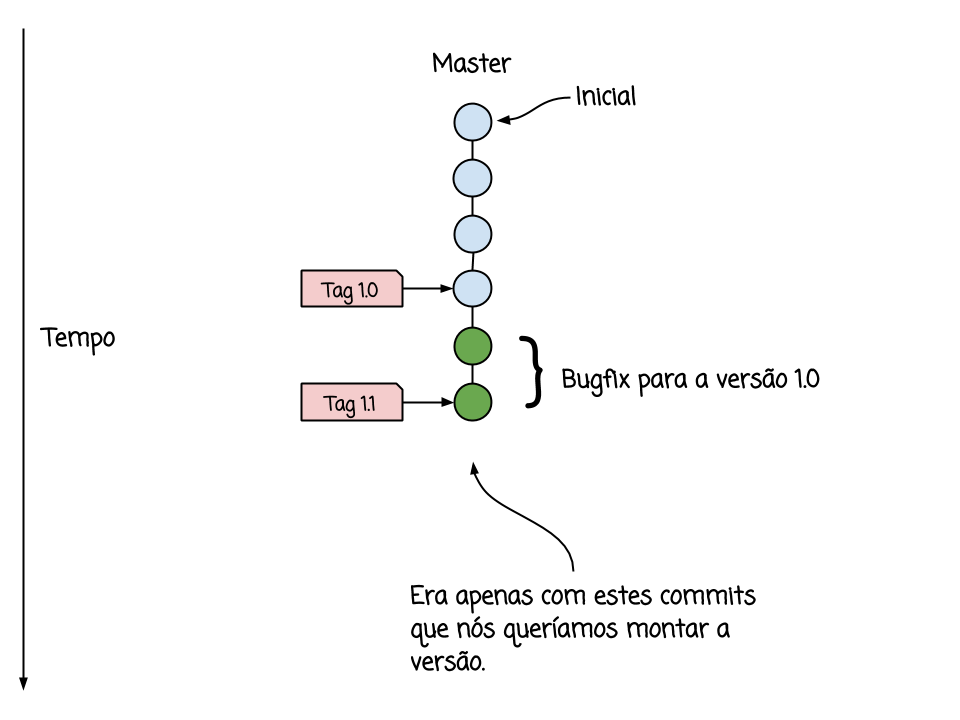
\includegraphics[width=1\textwidth]{img/exemplo-05}
\end{figure}
}
% 
% \section{Section no. 2} 
% \subsection{Lists I}
% \frame{\frametitle{unnumbered lists}
% \begin{itemize}
% \item Introduction to  \LaTeX  
% \item Course 2 
% \item Termpapers and presentations with \LaTeX 
% \item Beamer class
% \end{itemize} 
% }
% 
% \frame{\frametitle{lists with pause}
% \begin{itemize}
% \item Introduction to  \LaTeX \pause 
% \item Course 2 \pause 
% \item Termpapers and presentations with \LaTeX \pause 
% \item Beamer class
% \end{itemize} 
% }
% 
% \subsection{Lists II}
% \frame{\frametitle{numbered lists}
% \begin{enumerate}
% \item Introduction to  \LaTeX  
% \item Course 2 
% \item Termpapers and presentations with \LaTeX 
% \item Beamer class
% \end{enumerate}
% }
% \frame{\frametitle{numbered lists with pause}
% \begin{enumerate}
% \item Introduction to  \LaTeX \pause 
% \item Course 2 \pause 
% \item Termpapers and presentations with \LaTeX \pause 
% \item Beamer class
% \end{enumerate}
% }
% 
% \section{Section no.3} 
% \subsection{Tables}
% \frame{\frametitle{Tables}
% \begin{tabular}{|c|c|c|}
% \hline
% \textbf{Date} & \textbf{Instructor} & \textbf{Title} \\
% \hline
% WS 04/05 & Sascha Frank & First steps with  \LaTeX  \\
% \hline
% SS 05 & Sascha Frank & \LaTeX \ Course serial \\
% \hline
% \end{tabular}}
% 
% 
% \frame{\frametitle{Tables with pause}
% \begin{tabular}{c c c}
% A & B & C \\ 
% \pause 
% 1 & 2 & 3 \\  
% \pause 
% A & B & C \\ 
% \end{tabular} }
% 
% 
% \section{Section no. 4}
% \subsection{blocs}
% \frame{\frametitle{blocs}
% 
% \begin{block}{title of the bloc}
% bloc text
% \end{block}
% 
% \begin{exampleblock}{title of the bloc}
% bloc text
% \end{exampleblock}
% 
% 
% \begin{alertblock}{title of the bloc}
% bloc text
% \end{alertblock}
% }
\end{document}

